\documentclass{article}
\usepackage[T1]{fontenc} % codificação da fonte em 8-bits
\usepackage[utf8]{inputenc} % acentuação direta
\usepackage[brazil]{babel} % em portugues brasileiro
\usepackage[normalem]{ulem}
\useunder{\uline}{\ul}{}
\usepackage{graphicx}
\usepackage[utf8]{inputenc}
\usepackage{fullpage}
\usepackage{listings}
\usepackage{xcolor}
\usepackage{amsmath}
\usepackage{amssymb}
\usepackage{url}
\usepackage{hyperref}
\usepackage[linesnumbered,ruled,vlined]{algorithm2e}
% \usepackage{enumitem}
\usepackage[shortlabels]{enumitem}
\usepackage{listings}
\lstset { %
    language=C++,
    backgroundcolor=\color{black!5}, % set backgroundcolor
    basicstyle=\footnotesize,% basic font setting
}


\definecolor{mygreen}{rgb}{0,0.6,0}

% set the default code style
\lstset{
    language=C++,
    frame=tb, % draw a frame at the top and bottom of the code block
    tabsize=4, % tab space width
    showstringspaces=false, % don't mark spaces in strings
    numbers=none, % display line numbers on the left
    commentstyle=\color{mygreen}, % comment color
    keywordstyle=\color{blue}, % keyword color
    stringstyle=\color{red}, % string color
    backgroundcolor=\color{black!5}, % set backgroundcolor
    basicstyle=\footnotesize,% basic font setting
    literate = {-}{-}1, % <------ trick for '-' in shell commands
}

\parindent0in
\pagestyle{plain}
\thispagestyle{plain}

\newcommand{\assignment}{Lista 3}
\newcommand{\duedate}{April 08, 2022}


\title{Lista 3}
\date{}

\begin{document}

Fundação Getulio Vargas\hfill\\
Estruturas de Dados\hfill\textbf{\assignment}\\
Prof.\ Jorge Poco\hfill\textbf{Entrega:} \duedate\\
\smallskip\hrule\bigskip

{\let\newpage\relax\maketitle}
\maketitle

\section*{Parte 1 - Questões Teóricas}
\paragraph{Problema 1.} (16 pontos)

Considere a árvore AVL da \autoref{fig:avl-tree}.

\begin{figure}[h]
    \centering
    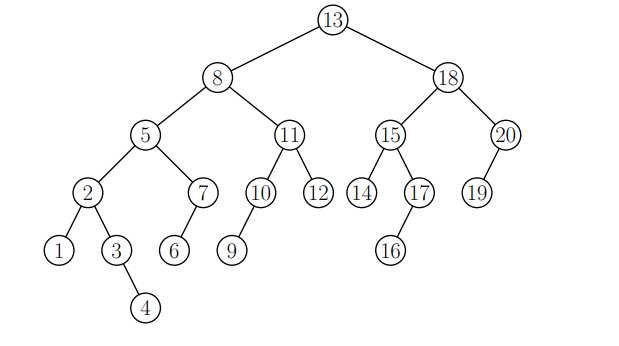
\includegraphics[width = 0.7\linewidth]{figures/fig-1.png}
    \caption{Exemplo de árvore AVL.}
    \label{fig:avl-tree}
\end{figure}

\begin{itemize}
    \item Desenhe a árvore novamente, indicando os fatores de balanceamento associados a cada nó.
    \item Mostre a árvore que resulta da operação \texttt{delete(19)}, após todo o rebalanceamento ter sido concluído. (Nós só precisamos da árvore final. Você pode fornecer intermediários resultados para crédito parcial.) 
\end{itemize}

\paragraph{Resposta 1}
 \begin{figure}[!h]
    \centering
    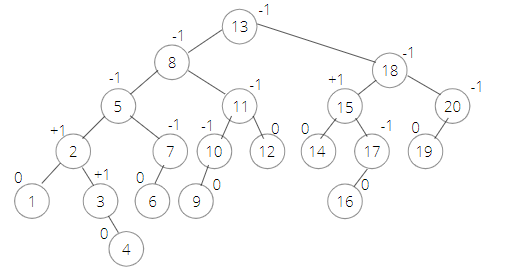
\includegraphics[width = 0.7\linewidth]{figures/img1.png}
    \caption{Resposta 1.1}
    \label{fig:aa-tree}
\end{figure}

 \begin{figure}[!h]
    \centering
    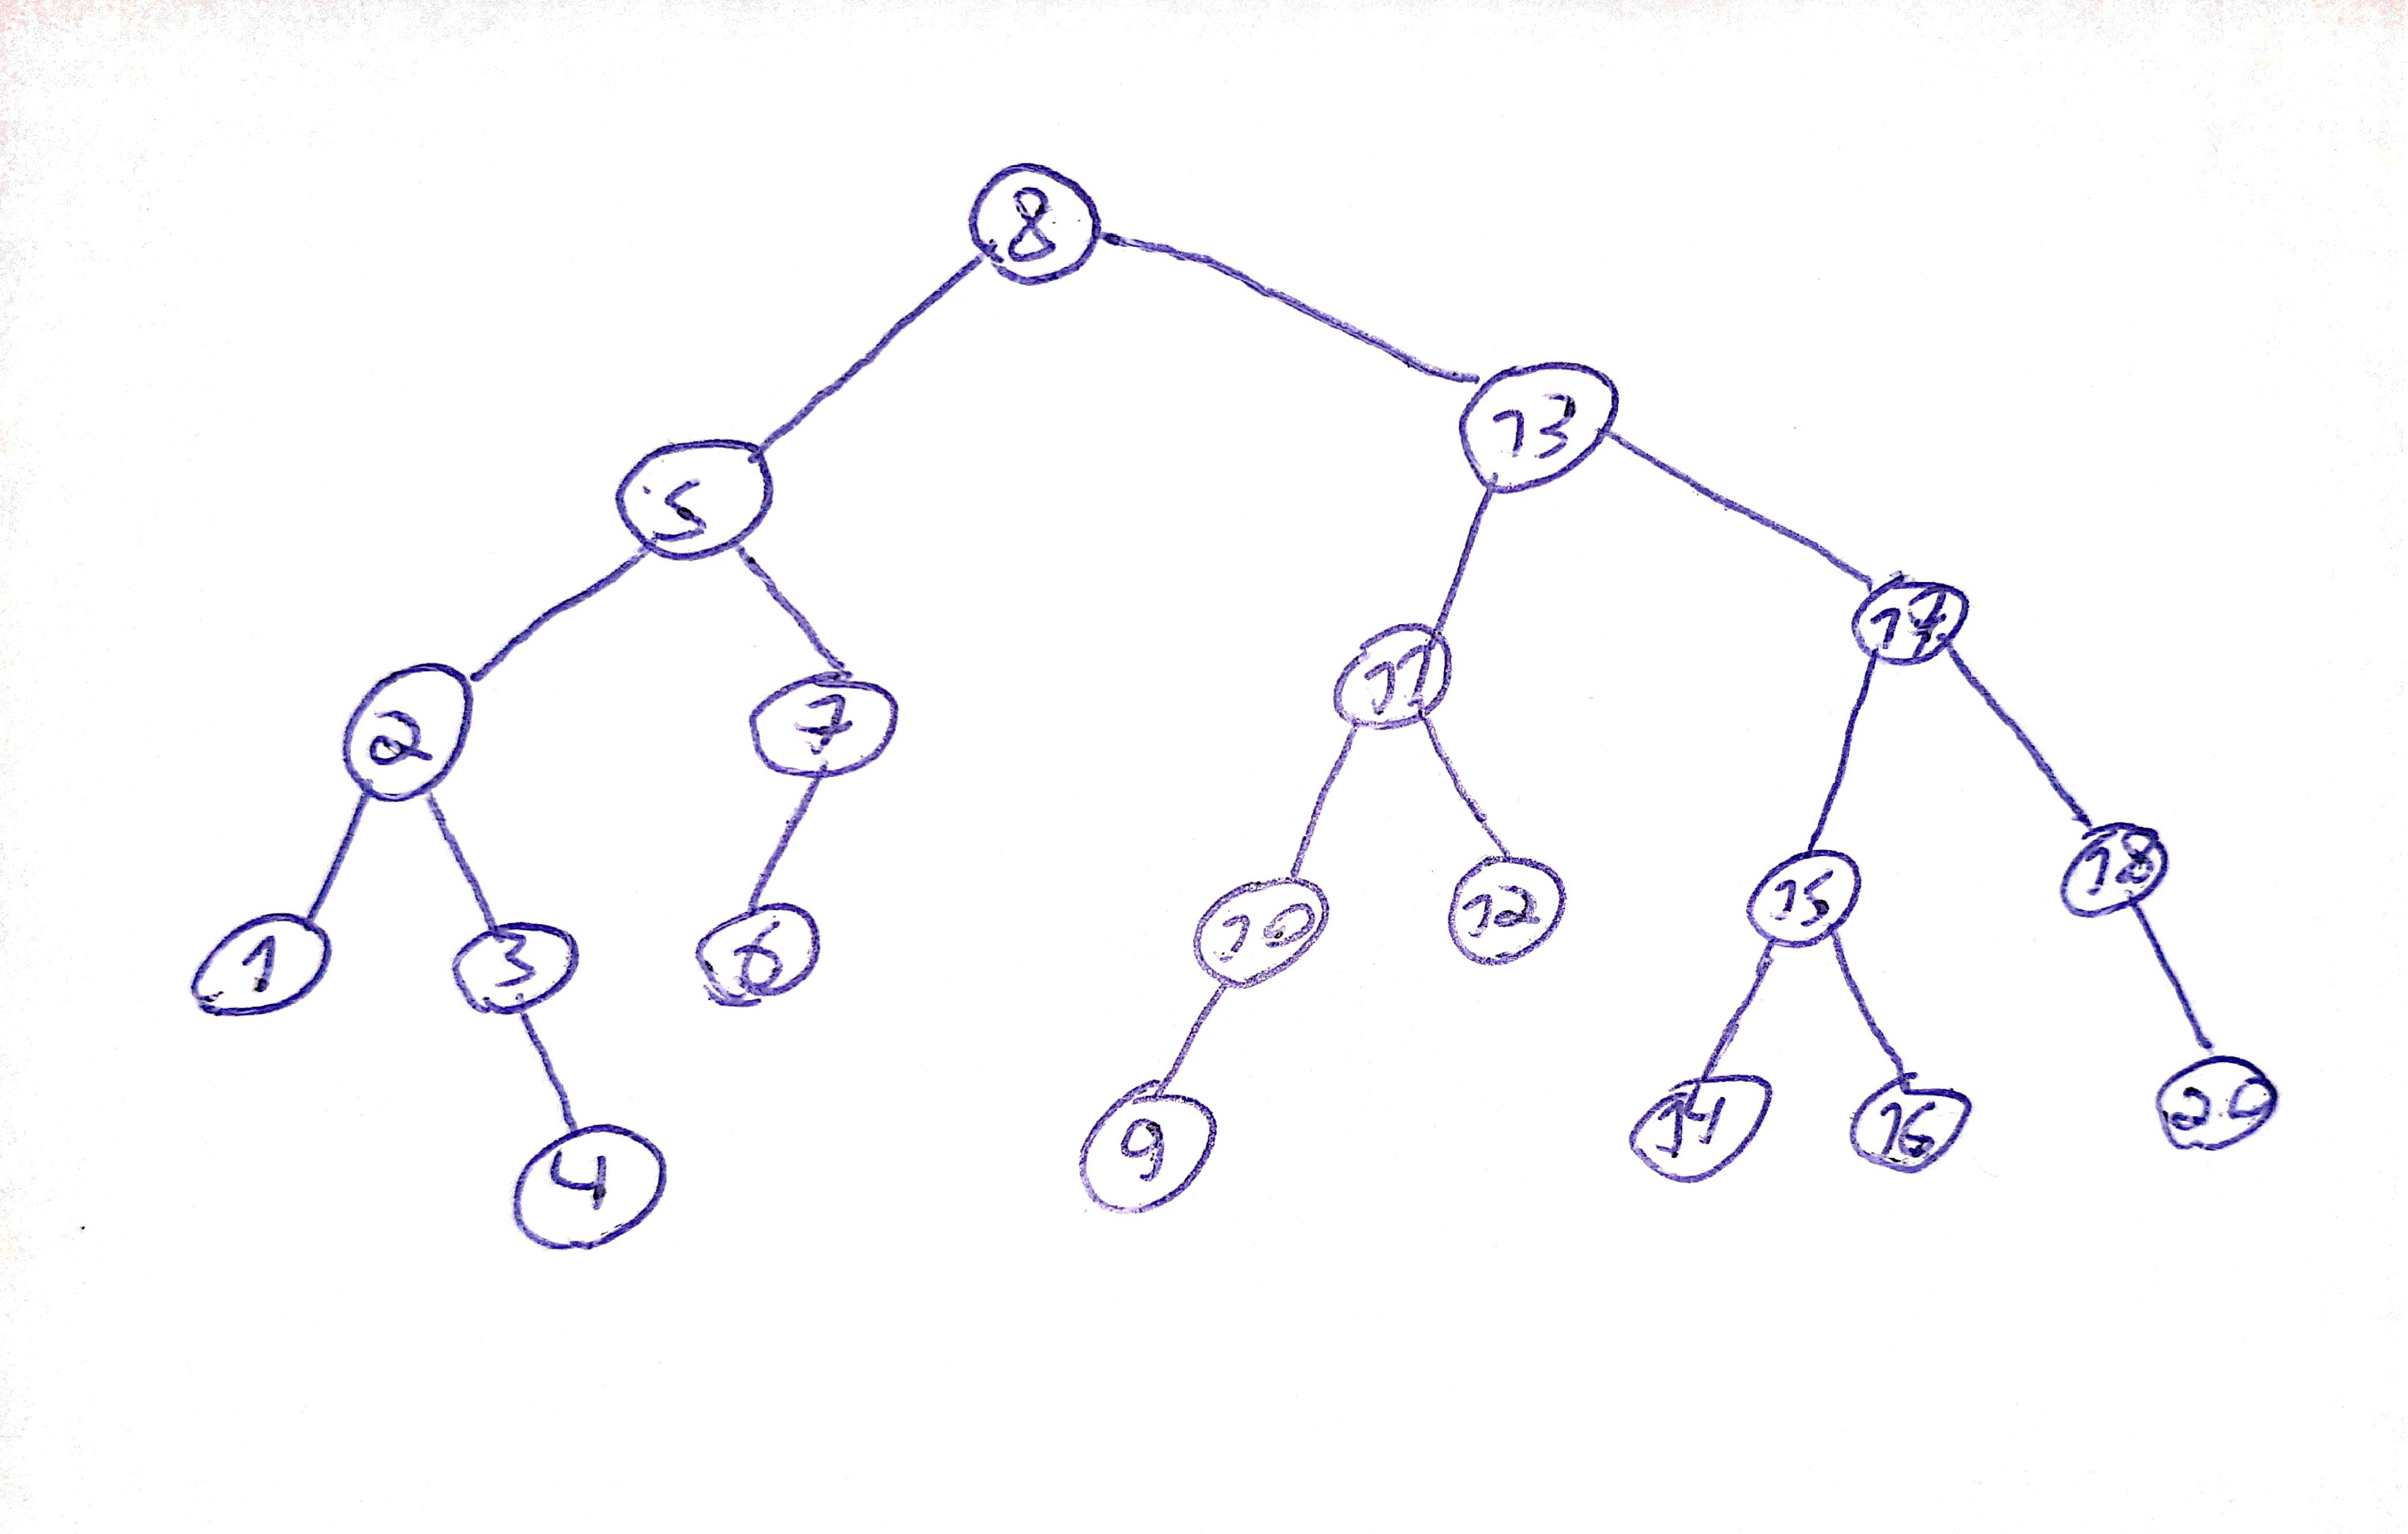
\includegraphics[width = 0.7\linewidth]{figures/img2.png}
    \caption{Resposta 1.2}
    \label{fig:aa-tree}
\end{figure}
\clearpage

\paragraph{Problema 2.} (16 pontos)
Considere a árvore AA da \autoref{fig:aa-tree}. Em ambos os casos, precisamos apenas da árvore final. Você pode fornecer resultados intermediários para crédito parcial.

\begin{figure}[h]
    \centering
    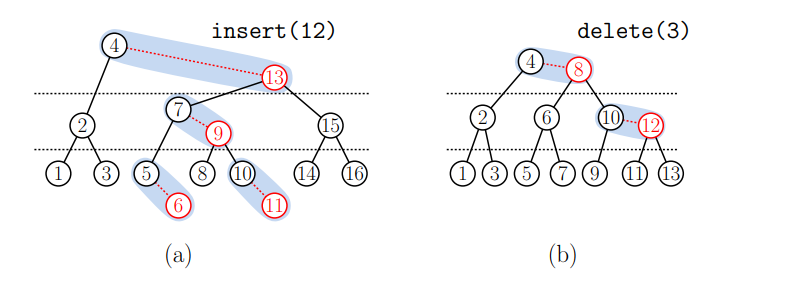
\includegraphics[width = 0.7\linewidth]{figures/fig-2.png}
    \caption{Exemplos de árvore AA.}
    \label{fig:aa-tree}
\end{figure}

\begin{itemize}
    \item Mostre o resultado da execução da operação \texttt{insert(12)} na árvore em \autoref{fig:aa-tree} (a).
    \item Mostre o resultado da execução da operação \texttt{delete(3)} da árvore em \autoref{fig:aa-tree} (b).
\end{itemize}

\paragraph{Resposta 2.}

\clearpage
 \begin{figure}[!h]
    \centering
    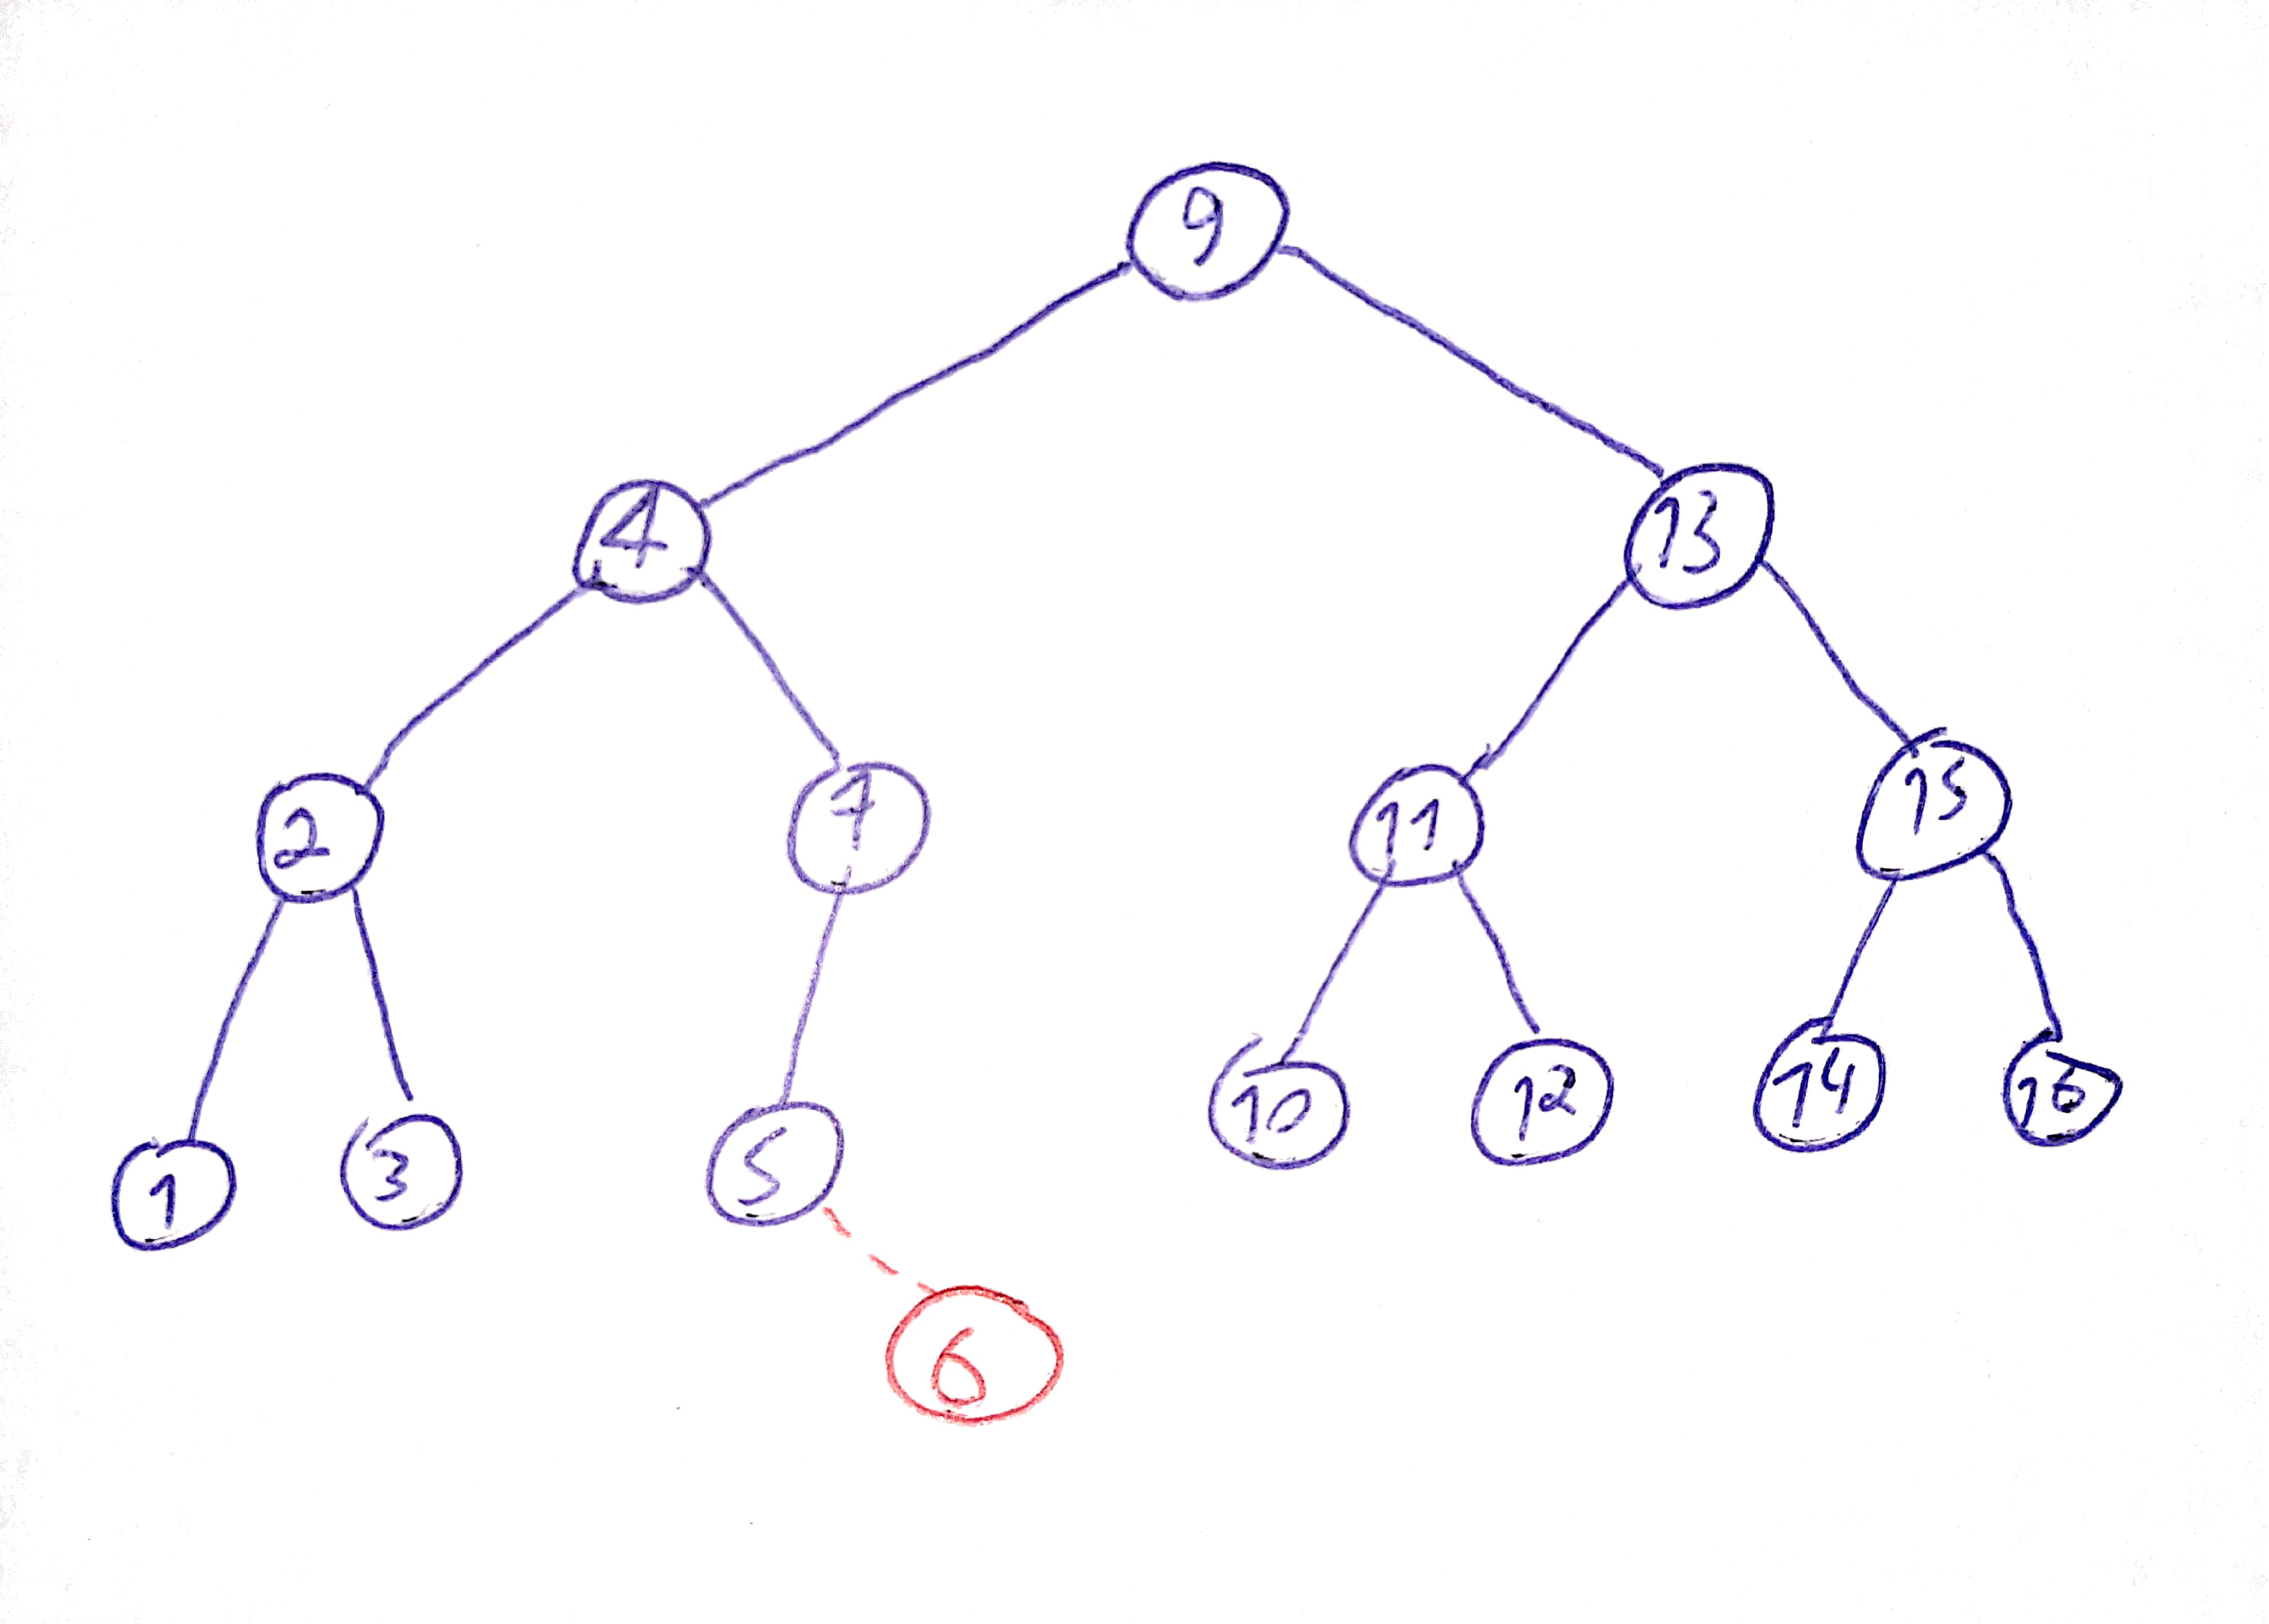
\includegraphics[width = 0.7\linewidth]{figures/img3.png}
    \caption{Resposta 2.1}
    \label{fig:aa-tree}
\end{figure}

 \begin{figure}[!h]
    \centering
    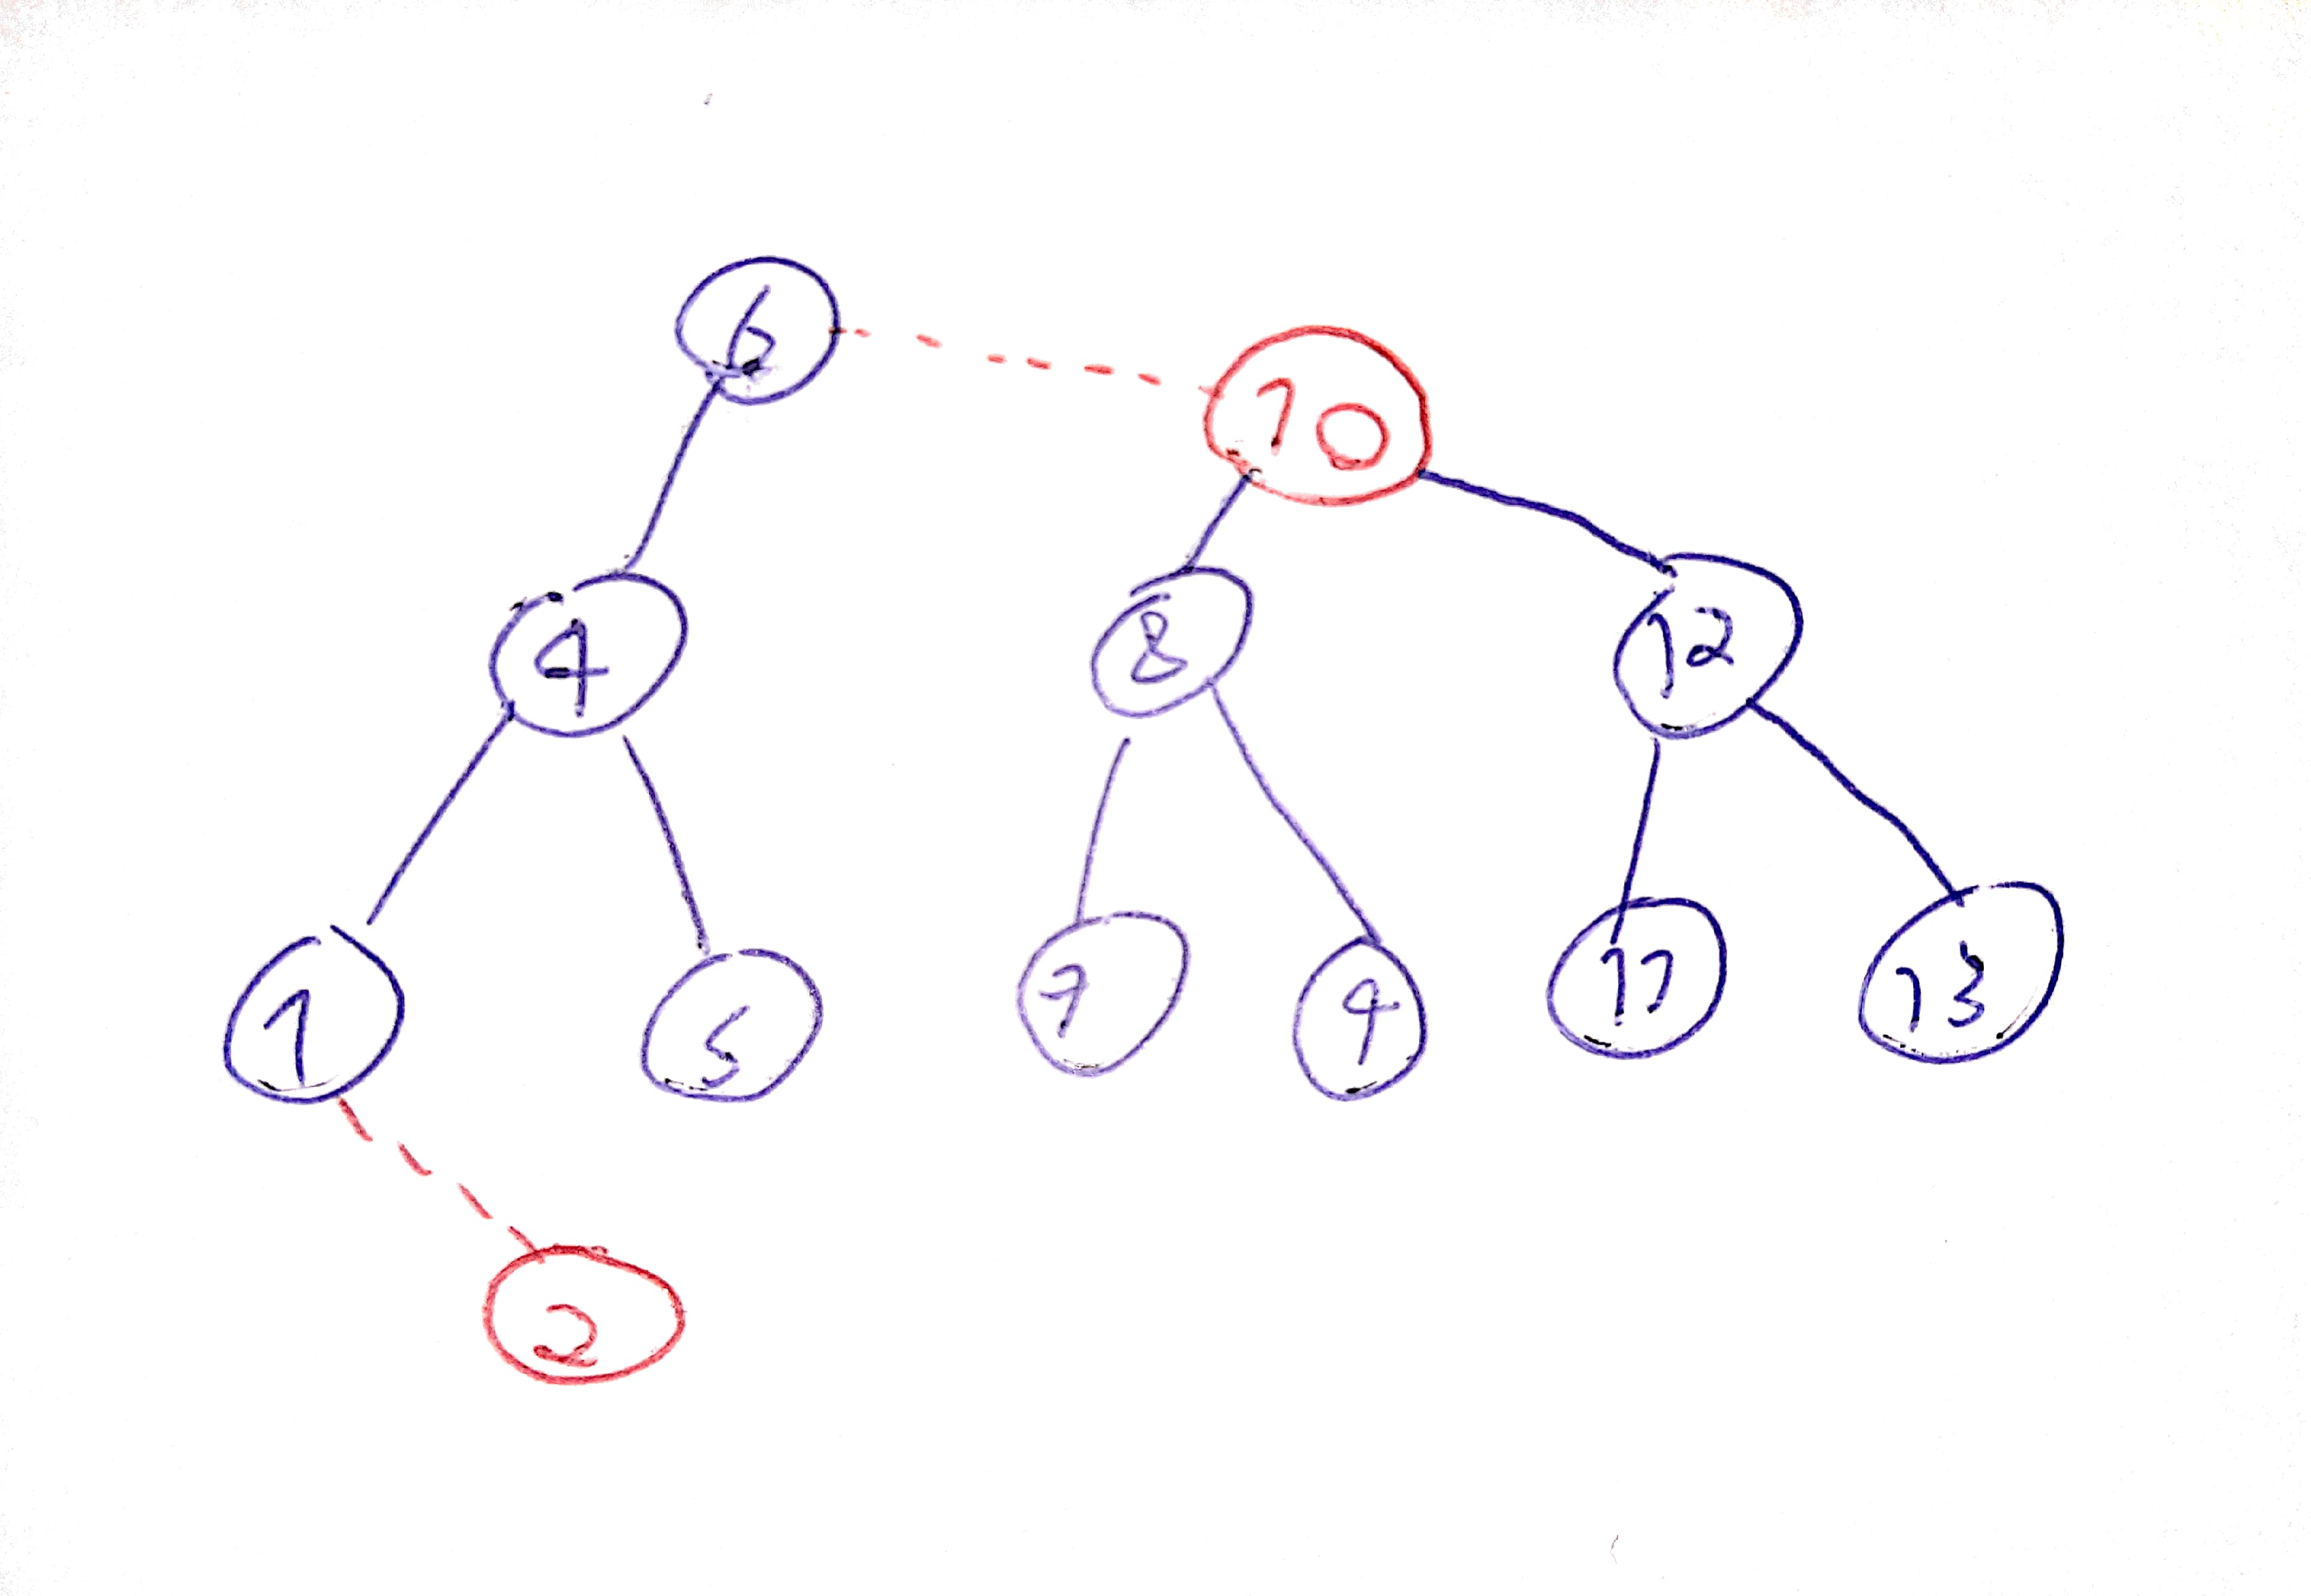
\includegraphics[width = 0.7\linewidth]{figures/img4.png}
    \caption{Resposta 2.2}
    \label{fig:aa-tree}
\end{figure}
\clearpage

\paragraph{Problema 3.} (18 pontos)
Em nossas implementações simples de árvore de busca binária, assumimos que cada nó armazena
apenas um par chave-valor (\texttt{p.key} e \texttt{p.value}) e ponteiros para os filhos esquerdo e direito do nó
(\texttt{p.left} e \texttt{p.right}). Na prática, muitas vezes é útil armazenar informações adicionais, incluindo
a seguir:

\begin{itemize}
    \item \texttt{p.parent}: pai de \texttt{p}, ou \texttt{null} se \texttt{p} for a raiz.;
    \item \texttt{p.min}: A menor chave na subárvore com raiz em \texttt{p};
    \item \texttt{p.max}: A maior chave na subárvore com raiz em \texttt{p};
    \item \texttt{p.size}: O número total de nós (incluindo \texttt{p}) na subárvore de \texttt{p}.
\end{itemize}

Modifique o pseudo-código de rotação à direita abaixo para que (além de
a rotação) todos os valores associados acima são atualizados. (Nota: Lembre-se que o
valor de retorno é significativo e deve permanecer \texttt{q}.)
\begin{lstlisting}
BinaryNode rotateRight(BinaryNode p) { 
    // rotacao a direita em p
    BinaryNode q = p.left;
    p.left = q.right;
    q.right = p;
    return q;
}
\end{lstlisting}

\paragraph{Resposta 3.}
\begin{lstlisting}
BinaryNode rotateRight(BinaryNode p) { 
    BinaryNode q = p.left;
    p.left = q.right;
    q.right = p;
    p.size = p.left.size + 1 + p.right.size;
    q.size = q.left.size + 1 + q.right.size;
    q.parent = p.parent;
    p.parent = q;
    p.max = p.right.max
    q.min = q.left.max
    return q;
}
\end{lstlisting}

\section*{Parte 2 - Tarefa de programação}

\paragraph{Quake Heaps:}

Este é a segunda parte da para implementar a \textit{Quake Heap}. Tal como acontece com \textit{heaps} padrão, esta estrutura de dados implementa uma fila de prioridade. Vamos relembrar os detalhes apresentados na lista 2.


\begin{figure}[!h]
    \centering
    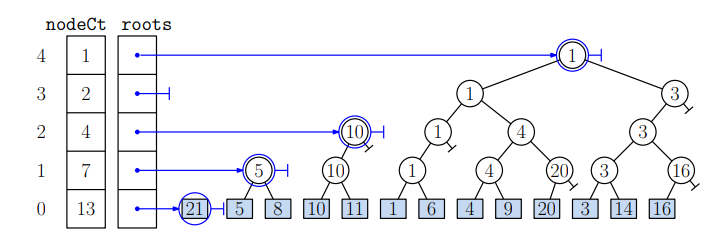
\includegraphics[width = 0.8\linewidth]{figures/fig1.png}
    \caption{Uma \textit{Quake Heap} armazenando as chaves $(21, 5, 8, 10, 11, 1, 6, 4, 9, 20, 3, 14, 16)$.}
    \label{fig:fig1}
\end{figure}

A \textit{QuakeHeap} suporta inserção e chaves decrescentes em tempo $O(1)$, e suporta \textit{extract-min} em $O(log n)$ tempo amortizado. 

A classe \texttt{QuakeHeap} funcionará com tipos genéricos, um tipo de chave
e um tipo de valor. O tipo de chave deve ser ordenável, e assumimos que ambos podem ser convertidos para strings com \texttt{to\_string}. 
O \texttt{QuakeHeap}  é representado como uma coleção de árvores binárias, onde cada nó armazena um par de valores-chave. Os nós dessas árvores são organizados em níveis. Todas as folhas residem no nível 0, e cada chave na \textit{heap} é armazenada em exatamente uma folha de alguma árvore. (Por exemplo, na \autoref{fig:fig1},
as chaves consistem nas 13 chaves nos nós de folha azul.)

Cada nó interno tem um filho esquerdo e um filho direito opcional. O valor da sua chave é igual ao do seu filho da esquerda. Se o filho direito existir, seu valor de chave será maior ou igual ao filho esquerdo. Cada raíz contém o menor valor de chave do que todas as folhas, que (pela nossa regra que a chave esquerda é menor) é o da folha mais à esquerda. Segue que a menor chave no \textit{heap} será armazenada em uma das raízes (mas geralmente não sabemos qual).

Cada nó armazena um par chave-valor, ponteiros filho esquerdo e direito, ponteiro pai e seu nível. 

Mantemos dois \texttt{arrays} adicionais organizados por nível:
\begin{itemize}
    \item \texttt{roots[lev]}: Uma lista encadeada contendo referências às raízes da árvore do nível \texttt{lev}. (Nós recomendo implementar isso como um lista encadeada de nós (\texttt{std::list})).
    \item \texttt{node\_counter[lev]}: Armazena o número total de nós no nível \texttt{lev}.
\end{itemize}

\texttt{Nodes} e \texttt{Locators}: Os principais objetos que estão sendo manipulados são os nós da \texttt{QuakeHeap}. Como mencionado acima, cada nó armazena um par chave-valor, links filho esquerdo e direito, link pai,
e seu nível na árvore. Os nós no nível 0 são folhas, portanto, ambos os links filho são nulos. Um nó raiz (em qualquer nível) tem um link pai de nulo. C++ fornece uma maneira elegante de definir uma classe aninhada a outra, assim faremos o \texttt{Node}, dentro da classe \texttt{QuakeHeap}.

Um detalhe complicado em qualquer estrutura de \textit{heap} que suporte diminuir o valor de uma chave é que precisamos de um mecanismo para identificar a entrada cuja chave desejamos diminuir. Quando inserimos um valor-chave
par, criamos um novo nó folha. Como o \texttt{Node} é um objeto protegido dentro do \texttt{QuakeHeap}, não podemos retornar um ponteiro diretamente para ele. Em vez disso, criamos um objeto público especial, chamado \texttt{Locator},
para incluir uma referência a este nó folha recém-inserido. A função \texttt{insert} retorna um localizador referenciando o nó recém-criado. 

\paragraph{Operações:} Para esta parte do projeto, começaremos implementando as funções básicas necessárias inserir chaves. Aqui está uma lista das operações que você deve implementar.

\begin{itemize}
    \item  \texttt{int GetMaxLevel(Locator loc)} (15 pontos): Dado um Locator \texttt{loc}, retorna determina a altura máxima de um nó "ancestral" alcançável seguindo a reversão dos links filho esquerdo na árvore. Por exemplo, para a \textit{heap} \autoref{fig:fig1}, o nível máximo da folha rotulada 21 é 0, o nível máximo de 4 é 2, o nível máximo de 1 é 4 e o nível máximo de 16 é 1.
    \item \texttt{T1 GetMinKey()} (15 pontos): Isso retorna a menor chave na heap e também reorganiza o heap, mesclando muitas pequenas árvores em uma grande árvore. As etapas são:
    \begin{itemize}
        \item Se o heap estiver vazio, lance uma Exception com a mensagem "Empty heap".
        \item Caso contrário, encontre a chave mínima no heap enumerando todos os nós em todas as listas de raízes, encontramos aquela com a menor chave. 
        \item Em seguida chame o processo MergeTree.
    \end{itemize}
    \item \texttt{void MergeTree()} (20 pontos): Consolida as árvores pelo seguinte processo. Itere o níveis de baixo para cima, de zero até o segundo nível mais alto (ou seja, \texttt{nLevels-2}). Em cada nível \texttt{k}:
    \begin{itemize}
        \item Ordene os nós de \texttt{roots[k]} em ordem crescente por suas chaves.
        \item Em seguida, mescle as árvores em pares da seguinte forma. Enquanto \texttt{roots[k]} tem pelo menos duas raízes:
        \begin{itemize}
            \item Extraia os dois primeiros nós raiz da lista ordenada. Chame-os de \texttt{u} e \texttt{v}. Já que a lista está ordenada, sabemos que \texttt{u.key <= v.key}.
            \item Crie um novo nó raiz \texttt{w}, com \texttt{u} como filho à esquerda e \texttt{v} como filho à direita. (Não esqueça de definir os links pai de \texttt{u} e \texttt{v} para apontar para \texttt{w}.) Por nossa convenção, a chave de \texttt{w} é defina como \texttt{u.key}. (Não nos importamos com o campo de valor de \texttt{w}. Você pode simplesmente defini-lo como \texttt{null}.)
            \item Adicione \texttt{w} às \texttt{raízes[k+1]}.
        \end{itemize}
    \item Observe que quando o processo da árvore de mesclagem é concluído, todos os níveis, exceto possivelmente o superior,
tem no máximo uma raiz. Isso é ilustrado na \autoref{fig:fig2}.
    \end{itemize}
\end{itemize}

\begin{figure}
    \centering
    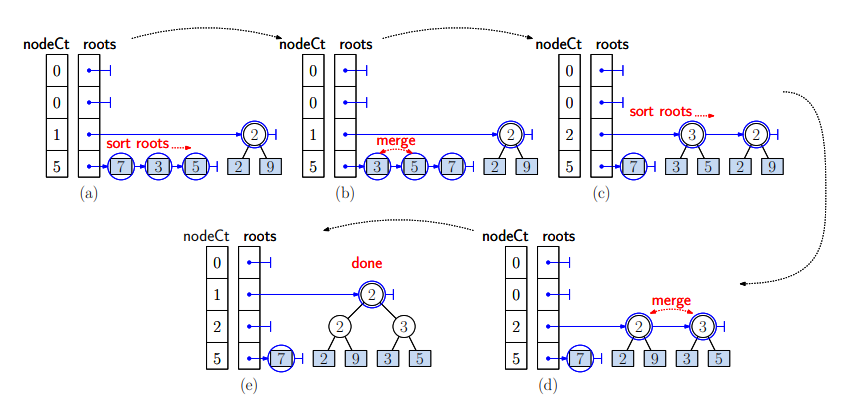
\includegraphics[width = \linewidth]{figures/fig2.png}
    \caption{Mesclando árvores. Trabalhando de baixo para cima, classificamos as raízes em cada nível e, em seguida, mesclamos pares consecutivos até que zero ou uma raiz permaneça.}
    \label{fig:fig2}
\end{figure}

Código base: Como na tarefa anterior, forneceremos o código esqueleto na classe no \textit{Github Classroom}. Iremos fornecer os arquivos \textit{headers} e o nosso \textit{tester} e os arquivos de texto de teste. Você só precisa implementar a \texttt{QuakeHeap} com as funções listadas acima. 

Nós vamos avaliar seu trabalho utilizando o seguinte comando para compilar:
\begin{lstlisting}[language=bash]
g++ -std=c++11 tester.cc -o tester
\end{lstlisting}

Caso o código não compile, a nota será 0.
Após a compilação, nós iremos realizar testes baseados em arquivos de texto (que estão dentro da pasta \texttt{src/tests}), utilizaremos o comando:

\begin{lstlisting}[language=bash]
tester <tests/test01-input.txt >tests/test01-output.txt
\end{lstlisting}
    
Com isso, será gerado um arquivo dentro da pastas tests de output, você deve comparar o \texttt{tests/test01-output.txt} com o arquivo \texttt{tests/test01-expected.txt} com o comando:

\begin{lstlisting}[language=bash]
diff tests/test01-output.txt tests/test01-expected.txt
\end{lstlisting}

Nós iremos considerar como um erro caso o comando \texttt{diff} aponte diferenças entre os arquivos (incluindo espaços em branco). 
O número 01 pode ser trocado por 02, 03, 04 e 05 para testar com os outros arquivos de teste. 

Uma outra avaliação será o estilo do código. Você deve formatar seu código baseado no estilo recomendo pelo  Google, de acordo com a referência no seguinte \href{https://google.github.io/styleguide/cppguide.html}{link}. 
%
Utilizaremos \textit{cpplint} para verificar o seu código. A cada \textit{alerta} referente a formatação, será retirado 5 pontos da nota. Você também pode verificar com as instruções no \href{https://github.com/cpplint/cpplint}{link}. Para executar, em um terminal use o comando:  

\begin{lstlisting}[language=bash]
cpplint --extensions=cc,hpp,h --header=h --repository=. tester.cc quake_heap.h quake_heap.hpp
\end{lstlisting}


\newpage
\appendix

\section{Detalhes avaliação}
Uma pergunta comum é "quanto detalhe é esperado nas respostas?", algumas orientações são:
%
\paragraph{Provar vs. Mostrar:}
Se lhe pedirmos para “provar” algo, estamos à procura de uma prova bem estruturada. Se você estiver aplicando a indução, tenha cuidado para distinguir seu(s) caso(s) básico(s) e indicar qual é a sua hipótese de indução. Se lhe pedirmos para “mostrar”, “explicar” ou “justificar”, estaremos geralmente apenas esperando uma explicação em português. Se você não tiver certeza, por favor, verifique.

\paragraph{Algoritmo vs. Pseudocódigo:} Quando pedimos um “algoritmo” estamos esperando uma descrição em alto nível de algum processo computacional, geralmente em uma combinação de português e notação matemática (por exemplo, “classifique as $n$ chaves e localize $x$ usando busca binária”). Para pseudocódigo, nós estão esperando uma descrição passo a passo mais detalhada que se pareça muito mais com C++ (por exemplo, “\texttt{Node q = p.left}”). Lembre-se de que você está escrevendo seu código para ser lido por um humano, e não por um compilador. Por favor, omita detalhes irrelevantes que são sintaxes de C++. Mesmo que não solicitemos explicitamente, sempre que você fornecer um algoritmo ou pseudocódigo, você deve sempre fornecer uma breve explicação em português. Isso ajuda o avaliador a entender quais são suas intenções, e se houver um pequeno erro em seu código, muitas vezes podemos usar seu explicação para entender quais eram suas reais intenções.

\end{document}

